\chapter{Introduction}
\label{chapter:intro}

With all the web services going into the cloud\cite{gartner}, service providers are starting to
have difficulties in maintaining their infrastructure with the available technologies.
This is shown by the increased interest in Software Defined Networking (SDN) \cite{sdn:whitepapers}.
SDN provides solutions for allowing a simple management of virtual networks devices by decoupling the control
plane from the data plane (or forwarding plane). This makes it easier to maintain configurations and network state
for a large number of systems. The switch control plane will be managed by a \texttt{controller},
and the data plane by a virtual or hardware switch. These two components will be presented in the following
sections.

\section{OpenFlow}

OpenFlow can be considered a model\cite{sdn} having various characteristics:
\begin{itemize}
 \item Communication protocols
 \item APIs for programatic configuration
 \item Separation between the control plane and the forwarding plane.
\end{itemize}

OpenFlow is the protocol which allows the separation between the network control plane and the forwarding plane.
It must be implemented both by a network device, like a switch, and by the controller. In this way it 
can communicate with any type of switch, whether it is a software or a hardware one. The controller becomes
the central point for configuration and management of the forwarding plane. This separation also, ideally, makes the
switch simpler. The reality can be a little different, because part of the functionality that is moved away from
the device is replaced by the OpenFlow implementation.

The required switch functions and the OpenFlow protocol are defined in an OpenFlow Specification.
This is maintained by the Open Networking Foundation\cite{onf}. At the time this project was developed, the specification
had reached version 1.4. The document defines the on-the-wire protocol format and various features that could
be implemented by switches.

Communication between OpenFlow controllers and switches is done using OpenFlow messages sent over the network.
Depending on the direction of the messages between a controller and a switch, these can be:
\begin{itemize}
 \item Controller to switch messages - For configuring the switch.
 \item Asynchronous messages - Sent by a switch without the controller asking for them. Used
 for signaling a state change or a packet arrival.
 \item Symmetric messages - Also sent without solicitation, but in any direction.
\end{itemize}

Each category contains many possible messages which evolve in time as a new specification version comes out.
Open vSwitch does not implement all of them and is not up to date with the latest specification. My objectives
were to work on some features for 1.3 and 1.4 version of the specification. These are better described in the following sections.


\section{Open vSwitch}
Open vSwitch\cite{ovs} is an implementation of a virtual software switch. Usually, a switch is implemented in hardware
with a management software on top of it. This provides a better performance for the critical operations
and still makes it flexible enough to be configured locally or remotely. However, nowadays this is not
enough. The dynamism of the current networks makes it harder to manage these switches. We must also
consider the fact that many services are now running in virtual machines which are already using
virtual switches.

Open vSwitch resembles the Linux software bridge. However, it has many more features which makes it
suitable in a large virtualized environment. It still provides standard protocols for port mirroring,
link aggregation, tunneling while leveraging the flexibility offered by the use of OpenFlow controllers.
The switch works by matching incoming traffic against flows installed by the controller and executing
the corresponding actions. A general architecture of this solution is shown in Figure~\ref{fig:genarch}.
The connection with the controller is not necessary to be separated from the production physical network
as depicted in Figure~\ref{fig:genarch}, but in that case, the switch must make sure not to apply the
same forwarding rules to both of them.

\begin{figure}
\begin{center}
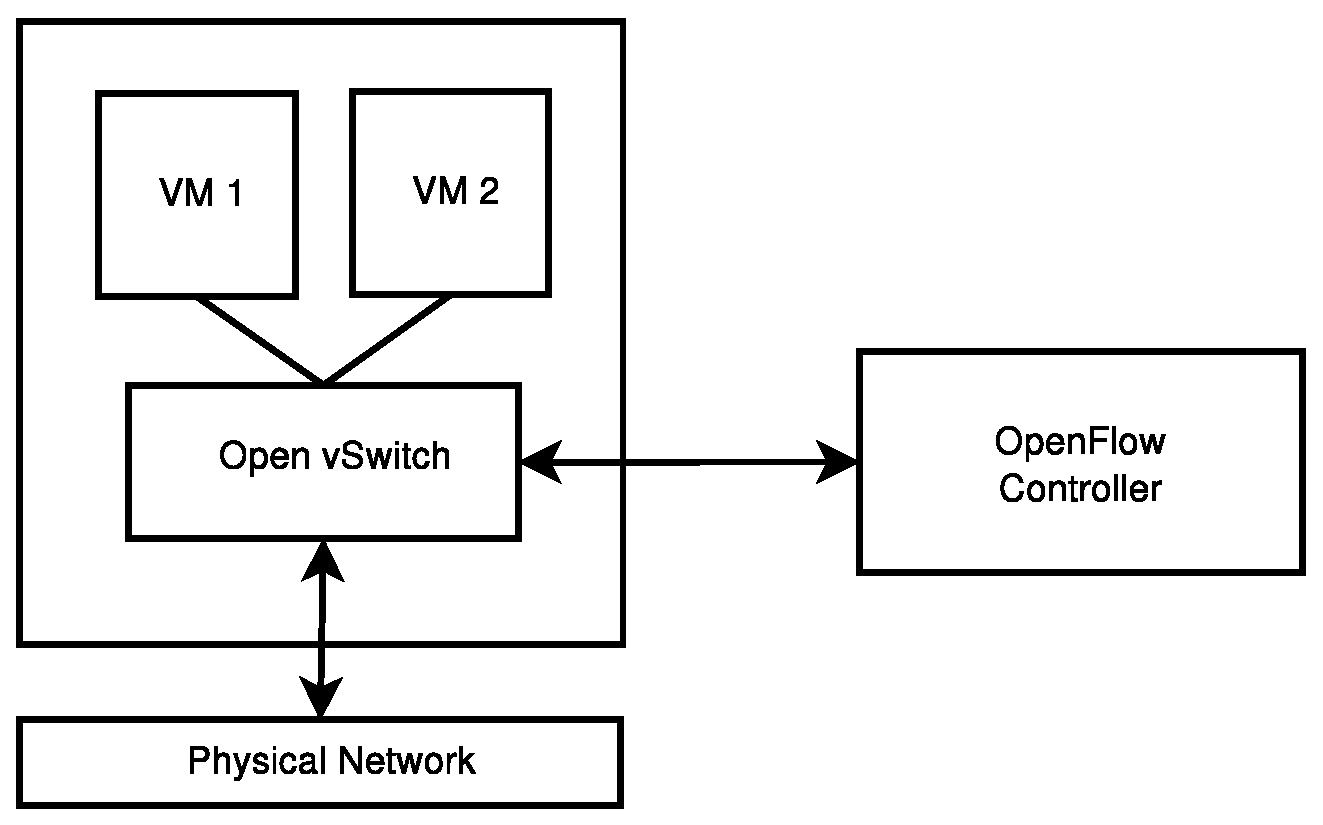
\includegraphics[scale=0.5]{src/img/ovs-arch.eps}
\end{center}
\caption{Using Open vSwitch With a Controller}
\label{fig:genarch}
\end{figure}

Rules used for matching traffic are named flows. Most Ethernet, IP and transport protocol fields can be used to
select incoming packets. Flows are installed in multiple flow tables linked together.
The switch has multiple physical or logical ports that can be used by OpenFlow. Processing of packets is done
in a pipeline formed by all the flow tables. A matched packet can be forwarded to an output port, but it can
also be sent to another table for further processing.

By default, Open vSwitch can work just like the Linux software bridge, without the need to use a controller.

\section{Project Description}
\label{sec:proj}

The flexibility introduced by Software Defined Networking and OpenFlow can also bring disadvantages. One
of them is related to the separation of the control plane from the data plane. Application controllers
need to have up to date information about the state of each of the switches that it controls in order to
make correct decisions.

One synchronization issue that can arise between switches and controllers is related to the permissions
that a controller has over the configuration of a switch. Because multiple controllers can connect to a
switch, the notion of \texttt{roles} has been introduced in OpenFlow.

We want to focus on implementing parts of the OpenFlow communication protocol that would improve
the synchronization between network devices and application controllers. In order to keep the solution
as simple as possible and make it standard across any OpenFlow device, we will implement it using
some of the newest features specified in OpenFlow 1.4.

Applying a set of multiple configuration changes regarding switch ports or forwarding rules can become
challenging when working with multiple switches. As part of this project, we will also design and implement
a solution that will allow atomic processing of OpenFlow message bundles.

As part of testing and development of the new OpenFlow 1.4 bundles feature, we will also implement a proof of concept
controller that should utilise this functionality. Together with an Intrusion Detection System like Snort\cite{snort}
we can create a flexible Intrusion Prevention System for virtualized hosts.

% \subsection{Project Scope}
% \label{sub-sec:proj-scope}

\subsection{Project Objectives}
\label{sub-sec:proj-objectives}

Firstly, it is necessary to develop an understaning of the inner workings of the virtual switch and the interractions
it has with a controller. Then, we'll design and implement several features from the specification that will
allow a better synchronization between the state of the switch with that of the controller. The final objective
is to integrate the changes of this project into the upstream Open vSwitch project. This also means to interact
with the Open vSwitch community for presenting the work, asking and doing patch reviews and getting the code in
the right shape for being accepted.


% \subsection{Related Work}
% \label{sub-sec:related-work}

